\chapter{Related Work}
\label{chapter:related-work}

This Chapter focuses on showcasing a series of works that should help the reader
understand what is the state of the different parts that compose the proposed
method presented in Chapter \ref{chapter:proposed-method}.

\section{Financial Forecasting}
\label{section:financial-forecasting}

\cite{Kadiri2015} This article presents findings of a questionnaire and an
interview survey on the perceived importance of chartist/technical and
fundamental analysis among foreign exchange traders and financial journalists in
Frankfurt, London, Vienna, and Zurich. Results confirm that most traders use
both forecasting approaches, and that the shorter the forecasting horizon, the
more important chartist/technical analysis is. Financial journalists put more
emphasis on fundamental analysis than do foreign exchange traders. Results
indicate that the importance of chartism may have increased over the last
decade. Regarding the use of chartist/technical and fundamental analysis on
seven forecasting horizons, four distinct clusters of traders can be
identified. Forecasting styles and the overall importance attached to
fundamental versus chartist/technical analysis vary across different trading
locations. Foreign exchange traders mention a series of psychological motives
and consequences of the use of chartism. Copyright © 2001 John Wiley & Sons,
Ltd.

\cite{Salganik2008} Individuals influence each others’ decisions about cultural
products such as songs, books, and movies; but to what extent can the perception
of success become a “self-fulfilling prophecy”? We have explored this question
experimentally by artificially inverting the true popularity of songs in an
online “music market,” in which 12,207 participants listened to and downloaded
songs by unknown bands. We found that most songs experienced self-fulfilling
prophecies, in which perceived—but initially false—popularity became real over
time. We also found, however, that the inversion was not self-fulfilling for the
market as a whole, in part because the very best songs recovered their
popularity in the long run. Moreover, the distortion of market information
reduced the correlation between appeal and popularity, and led to fewer overall
downloads. These results, although partial and speculative, suggest a new
approach to the study of cultural markets, and indicate the potential of
web-based experiments to explore the social psychological origin of other
macro-sociological phenomena.

\cite{Castillo2001} We describe in this paper the application of several neural
network architectures to the problem of simulating and predicting the dynamic
behavior of complex economic time series. We use several neural network models
and training algorithms to compare the results and decide at the end which one
is best for this application. We also compare the simulation results with fuzzy
logic models and the traditional approach of using a statistical model. In this
case, we use real time series ofprices of consumer goods to test our
models. Real prices of tomato and green onion in the US. show complex
fluctuations in time and are very complicated to predict with traditional
statistical approaches. For this reason, we have chosen neural networks and
fuzzy logic to simulate and predict the evolution of these prices in the
U. S. market.

\cite{melin2007hybrid} We describe in this paper the application of a modular
neural network architecture to the problem of simulating and predicting the
dynamic behavior of complex economic time series. We use several neural network
models and training algorithms to compare the results and decide at the end,
which one is best for this application. We also compare the simulation results
with the traditional approach of using a statistical model. In this case, we use
real time series of prices of consumer goods to test our models. Real prices of
tomato in the U.S. show complex fluctuations in time and are very complicated to
predict with traditional statistical approaches. For this reason, we have chosen
a neural network approach to simulate and predict the evolution of these prices
in the U.S. market.

\cite{Cai2013} Stock market has been developed for over twenty years, and has
gone deeply into all aspects of daily economic life and attracted more and more
investors’ attentions. Therefore, researches on finding internal rules and
establishing an efficient stock forecast model to help investors minimize risks
and maximize returns are very practical and amazing. In this paper, a hybrid
model FTSGA based on fuzzy time series and genetic algorithm is proposed. FTSGA
improves the performance by applying the operations of genetic algorithm such as
selection, crossover and mutation to iteratively search a good discourse
partition. TAIEX is selected as the experimental data set. And experimental
results show that comparing with other models based on fuzzy time series FTSGA
can greatly reduce the root mean square error and improve accuracy.

\cite{Gamil2007} —this paper proposes a multi agent and fuzzy logic based DSS
for stock market. This system will help investors of the stock market to take
the correct buy/sell/hold decisions. The results obtained from the proposed
fuzzy logic model were satisfactory but not accurate. A fuzzy tuning methodology
was introduced to enhance the accuracy of the decisions. The tuning methodology
which uses genetic algorithms is presented also in this paper. A multi agent
framework is proposed for the implementation of the system. Experimental
simulation using actual price data form NASDAQ index is carried out to
demonstrate the power of the proposed model.

\cite{Ijegwa2014} Decision making process in stock trading is a complex
one. There are numbers of technical indicators that are used by traders to study
trends of the market and make buying and selling decisions based on their
observations. This research seeks to deploy fuzzy inference to stock market,
with four indicators used in technical analysis to aid in the decision making
process in order to deal with probability. The four technical indicators are the
Moving Average Convergence/Divergence (MACD), Relative Strength Index (RSI),
Stochastic Oscillator (SO) and On-Balance Volume (OBV). The fuzzy rules are a
combination of the trading rules for each of the indicators used as the input
variables of the fuzzy system and for all the four technical indicators used,
the membership functions were also defined. The result is a recommendation to
buy, sell or hold. Data were collected for two Nigerian banks for testing and
evaluation of the system. The technical indicators were then computed for each
data and from the computed technical indicators; experiment was carried out for
two months. The system generated satisfactory recommendation as when to buy,
sell or hold, when the output is compared with actual data collected from the
Nigerian Stock Exchange. The system can therefore act as an effective model for
traders in the stock market when there is a combination of the recommendation
with the individual’s trading skills.

\cite{Garcia-Almanza2006} In recent years the computers have shown to be a
powerful tool in financial forecasting. Many machine learning techniques have
been utilized to predict movements in financial markets. Machine learning
classifiers involve ex- tending the past experiences into the future. However
the rareness of some events makes difficult to create a model that detect
them. For example bubbles burst and crashes are rare cases, however their
detection is crucial since they have a significant impact on the investment. One
of the main problems for any machine learning classifier is to deal with
unbalanced classes. Specifically Genetic Pro- gramming has limitation to deal
with unbalanced environments. In a previous work we described the Repository
Method, it is a technique that analyses deci- sion trees produced by Genetic
Programming to discover classification rules. The aim of that work was to
forecast future opportunities in financial stock markets on situations where
positive instances are rare. The objective is to extract and collect different
rules that classify the positive cases. It lets model the rare instances in
different ways, increasing the possibility of identifying similar cases in the
future. The objective of the present work is to find out the factors that work
in favour of Repository Method, for that purpose a series of experiments was
performed.

\cite{Connor2005} The aim of this study is to evaluate the effectiveness of
using external indicators, such as commodity prices and currency exchange rates,
in predicting movements in the Dow Jones Industrial Average index. The
performance of each technique is evaluated using different domain specific
metrics. A comprehensive evaluation procedure is described, involving the use of
trading simulations to assess the practical value of predictive models, and
comparison with simple benchmarks that respond to underlying market growth. In
the experiments presented here, basing trading decisions on a neural network
trained on a range of external indicators resulted in a return on investment of
23.5\% per annum, during a period when the DJIA index grew by 13.03\% per
annum. A substantial dataset has been compiled and is available to other
researchers interested in analysing financial time series.

%% curve-fitting
In several efforts, researchers create regression models using technical or
fundamental indicators as training datasets. Examples of regression techniques
are autoregression \cite{burg1968new}, symbolic regression
\cite{billard2002symbolic}, and linear regression \cite{kutner2004applied}.


%% preprocessing
The work by Lu, Lee, and Chiu \cite{Lu2009} point out the complexity of
financial time-series. They note its noisy nature and propose a technique to
reduce this noise based in a two-stage modeling approach using Independent
Component Analysis (ICA) and Support Vector Regression (SVR). Their approach
first uses ICA for generating independent components to identify and remove
those containing the noise, then the remaining components are used to
reconstruct the forecasting variables which now contain less noise and are the
input of the SVR forecasting model.


%% neural networks
Lastly, it is imperative to mention the use of Neural Networks in regression
tasks, as it is a technique that has been proved to be very effective for this
kind of problems. O'Connor and Madden \cite{Connor2005} obtained some remarkable
results where they obtained an annual 23.5\% of Rate of Investment on Dow Jones
data used for training and testing. Another example is given by Castillo and
Melin \cite{castillo2001simulation}, where they compare different hybrid
architectures that combine Neural Networks and Fuzzy Logic for the prediction of
financial time-series.

\section{Interpretation of Financial Markets}
\label{section:interpretation-of-financial-markets}

\cite{Brown2013} This research uses a Niche Genetic Algorithm (NGA) called
Dynam- ic-radius Species-conserving Genetic Algorithm (DSGA) to select stocks to
purchase from the Dow Jones Index. DSGA uses a set of training data to produce a
set of rules. These rules are then used to predict stock prices. DSGA is an NGA
that uses a clustering algorithm enhanced by a tabu list and radial
variations. DSGA also uses a shared fitness algorithm to investigate different
areas of the domain. This research applies the DSGA algorithm to training data
which produces a set of rules. The rules are applied to a set of testing data to
obtain results. The DSGA algorithm did very well in predicting stock movement.

%% market interpretability
The work by Brown, Pelosi and Dirska uses a Niche Genetic Algorithm called
Dynamic-radius Species-conserving Genetic Algorithm (DSGA) to select stocks to
purchase from the Dow Jones Index.

%% decision support systems

\cite{Keen1980} general theory about decision support systems.

\cite{Tsang2004} Evolutionary Dynamic Data Investment Evaluator (EDDIE) is a
genetic programming (GP)-based decision support tool for financial
forecasting. EDDIE itself does not replace forecasting experts. It serves to
improve the productivity of experts in searching the space of decision trees,
with the aim to improve the odds in its user’s favour. The efficacy of EDDIE has
been reported in the literature. However, discovering patterns in historical
data is only the first step towards building a practical financial forecasting
tool. Data preparation, rules organization and application are all important
issues. This paper describes an architecture that embeds EDDIE for learning from
and monitoring the stock market.

\cite{tsang1998eddie} Investment involves the maximisation of return on one’s
investment whilst minimising risk. Good forecasting, which often requires expert
knowledge, can help to reduce risk. In this paper, we propose a genetic
programming based system EDDIE, (which stands for Evolutionary Dynamic Data
Investment Evaluator), as a forecasting tool. Genetic programming is inspired by
evolution theory, and has been demonstrated to be successful in other
areas. EDDIE interacts with the users and generates decision trees, which can
also be seen as rule sets. We argue that EDDIE is suitable for forecasting
because apart from utilising the power of genetic programming to efficiently
search the space of decision trees, it allows expert knowledge to be channelled
into forecasting and it generates rules which can easily be understood and
verified. EDDIE has been applied to horse racing and achieved outstanding
results. When experimented on 180 handicap races (real data) in the UK, it
out-performed other common strategies used in horse race betting by great
margins. The idea was then extended to financial forecasting. When tested on
historical S&P-500 data EDDIE achieved a respectable annual rate of return over
a three and a half year period. While luck may play a part in the success of
EDDIE, our experimental results do indicate that EDDIE is a tool which deserves
more research.

\cite{Sprague1980} This article proposes This article proposes a framework to a
framework to explore explore the the nature, scope, nature, scope, and content
of the evolving topic of and content of the evolving topic of Decision Support
Systems (DSS). The first part of the Decision Support Systems (DSS). The first
part of the framework considers framework considers (a) three levels (a) three
levels of technology of technology which have been designated DSS, (b) the
developmen- which have been designated DSS, (b) the developmen- tal approach
that is evolving for the creation of a DSS, tal approach that is evolving for
the creation of a DSS, and (c) the roles of several key types of people in the
and (c) the roles of several key types of people in the building and use of a
DSS. The second part develops a building and use of a DSS. The second part
develops a descriptive model to assess descriptive model to assess the
performance objec- the performance objec- tives and the capabilities of a DSS as
viewed by three of tives and the capabilities of a DSS as viewed by three of the
major participants in their continued development the major participants in
their continued development and use. The final section outlines several issues
in the and use. The final section outlines several issues in the future growth
and development of a DSS as a potentially future growth and development of a DSS
as a potentially valuable type of information system in organizations.

% Technical analysis
\cite{Achelis2000} general theory about technical analysis.

\cite{Nison1991} general theory about japanese candlesticks and patterns.

\cite{Wilder1978} theory about his technical indicators.

\cite{Blume1994} We investigate the informational role of volume and its
applicability for technical analysis. We develop a new equilibrium model in
which aggregate supply is fixed and traders receive signals with differing
quality. We show that volume provides information on information quality that
cannot be deduced from the price statistic. We show how volume, information
precision, and price movements relate, and demonstrate how sequences of volume
and prices can be informative. We also show that traders who use information
contained in market statistics do better than traders who do not. Technical
analysis thus arises as a natural component of the agents’ learning process.

\cite{Lo2000} Technical analysis, also known as “charting,” has been a part of
financial practice for many decades, but this discipline has not received the
same level of academic scrutiny and acceptance as more traditional approaches
such as fundamental analy- sis. One of the main obstacles is the highly
subjective nature of technical analy- sis—the presence of geometric shapes in
historical price charts is often in the eyes of the beholder. In this paper, we
propose a systematic and automatic approach to technical pattern recognition
using nonparametric kernel regression, and we apply this method to a large
number of U.S. stocks from 1962 to 1996 to evaluate the effectiveness of
technical analysis. By comparing the unconditional empirical dis- tribution of
daily stock returns to the conditional distribution—conditioned on spe- cific
technical indicators such as head-and-shoulders or double-bottoms—we find that
over the 31-year sample period, several technical indicators do provide incre-
mental information and may have some practical value.

\cite{Neely1997} Using genetic programming techniques to find technical trading
rules, we find strong ev- idence of economically significant out-of-sample
excess returns to those rules for each of six exchange rates over the period
1981–1995. Further, when the dollar/Deutsche mark rules are allowed to determine
trades in the other markets, there is significant improve- ment in performance
in all cases, except for the Deutsche mark/yen. Betas calculated for the returns
according to various benchmark portfolios provide no evidence that the returns
to these rules are compensation for bearing systematic risk. Bootstrapping
results on the dollar/Deutsche mark indicate that the trading rules detect
patterns in the data that are not captured by standard statistical models.

Taylor, Mark and Allen, Helen \cite{Fund1992} Technical, or chartist, analysis of
financial markets involves providing forecasts or trading advice on the basis of
largely visual inspection of past prices, without regard to any underlying
economic or 'fundamental' analysis. This paper reports the results of a
questionnaire survey, conducted on behalf of the Bank of England, among chief
foreign exchange dealers based in London in November 1988. Amongst other
findings, it is revealed that at least 90 per cent of respondents place some
weight on this form of non-fundamental analysis when forming views at one or
more time horizons. There is also a skew towards reliance on technical, as
opposed to fundamentalist, analysis at shorter horizons, which becomes steadily
reversed as the length of horizon considered is increased. A very high
proportion of chief dealers view technical and fundamental analysis as
complementary forms of analysis and a substantial proportion suggest that
technical advice may be self-fulfilling.

% Agents

\cite{Bundesbank2007} This review deals with several microscopic (“agent-based”) models
of financial markets which have been studied by economists and physi- cists over
the last decade: Kim-Markowitz, Levy-Levy-Solomon, Cont- Bouchaud,
Solomon-Weisbuch, Lux-Marchesi, Donangelo-Sneppen and Solomon-Levy-Huang. After
an overview of simulation approaches in financial economics, we first give a
summary of the Donangelo- Sneppen model of monetary exchange and compare it with
related models in economics literature. Our selective review then outlines the
main ingredients of some influential early models of multi-agent dynamics in
financial markets (Kim-Markowitz, Levy-Levy-Solomon). As will be seen, these
contributions draw their inspiration from the complex appearance of investors’
interactions in real-life markets. Their main aim is to reproduce (and, thereby,
provide possible explana- tions) for the spectacular bubbles and crashes seen in
certain histori- cal episodes, but they lack (like almost all the work before
1998 or so) a perspective in terms of the universal statistical features of
financial time series. In fact, awareness of a set of such regularities
(power-law tails of the distribution of returns, temporal scaling of volatility)
only gradually appeared over the nineties.

\cite{Grothmann2002} general theory about multi agent systems in market
modelling using neural networks.

\cite{Lebaron2001} a builder's guide to agent based financial markets.

\cite{Klingert2017} Prediction markets are an interesting instrument to draw on
the "wisdom of the crowds", e.g., to forecast sales or project risks. So far,
mainly two market mechanisms have been implemented in prediction markets, the
continuous double auction and logarithmic market scoring rule. However, the
effects of the choice between these two market mechanisms on relevant variables
such as prediction market accuracy are not fully understood. These effects are
relevant as faulty prediction market outcomes might cause wrong decisions. This
work contributes via an experiment-based simulation model to understand the
mechanism-related effects and to direct further laboratory experiments. Our
results show, that the mechanism decision does matter. Due to the higher amount
of trades and the lower standard deviation of the price, the logarithmic market
scoring rule seems to have a clear advantage on a first view. Taking the
accuracy error as an independent variable, the effects are not as
straightforward and depend on the environment and actors.

\cite{Sherstov2005} This paper documents the development of three autonomous
stock- trading agents within the framework of the Penn Exchange Simulator (PXS),
a novel stock-trading simulator that takes advantage of electronic crossing net-
works to realistically mix agent bids with bids from the real stock market
[1]. The three approaches presented take inspiration from reinforcement
learning, myopic trading using regression-based price prediction, and market
making. These ap- proaches are fully implemented and tested with results
reported here, including individual evaluations using a fixed opponent strategy
and a comparative analysis of the strategies in a joint simulation. The
market-making strategy described in this paper was the winner in the fall 2003
PLAT live competition and the runner- up in the spring 2004 live competition,
exhibiting consistent profitability. The strategy's performance in the live
competitions is presented and analyzed.

\cite{Chen2001} In this paper, we propose a new architecture to study artificial
stock markets. This architecture rests on a mechanism called 'school' which is a
procedure to map the phenotype to the genotype or, in plain English, to uncover
the secret of success. We propose an agent-based model of 'school', and consider
school as an evolving population driven by single-population GP (SGP). The
architecture also takes into consideration traders' search behavior. By
simulated annealing, traders' search density can be connected to psychological
factors, such as peer pressure or economic factors such as the standard of
living. This market architecture was then implemented in a standard artificial
stock market. Our econometric study of the resultant artificial time series
evidences that the return series is independently and identically distributed
(iid), and hence supports the efficient market hypothesis (EMH). What is
interesting though is that this iid series was generated by traders, who do not
believe in the EMH at all. In fact, our study indicates that many of our traders
were able to find useful signals quite often from business school, even though
these signals were short-lived.

\cite{Pellizzari2007} We compare price dynamics of different market protocols
(batch auction, continuous double auction and dealership) in an agent-based
artificial exchange. In order to distinguish the effects of market architectures
alone, we use a controlled environment where allocative and informational issues
are neglected and agents do not optimize or learn. Hence, we rule out the
possibility that the behavior of traders drives the price dynamics. Aiming to
compare price stability and execution quality in broad sense, we analyze
standard deviation, excess kurtosis, tail exponent of returns, volume, perceived
gain by traders and bid-ask spread. Overall, a dealership market appears to be
the best candidate, generating low volume and volatility, virtually no excess
kurtosis and high perceived gain.



\subsection{Technical Analysis}
\label{subsection:technical-analysis}

\section{Preprocessing of Financial Market Data}
\label{section:preprocessing-of-financial-market-data}

\section{Multi-agent Systems}
\label{section:multi-agent-systems}

The core algorithm of the proposed method is, at its highest level, a
multi-agent system.

Klingert and Meyer \cite{Klingert_2012} implement a multi-agent system to
analyze the effect of two market mechanisms: the continuous double auction and
logarithmic market scoring rule. The purpose of the agent-based simulation model
is to see the effect on the number of trades, the accuracy of prediction markets
and the standard deviation of the prices in order to prove three hypothesis that
they propose. In the end, due to a higher amount of trades and lower standard
deviation of the price, their results indicate that the logarithmic market
scoring rule seems to have an advantage over the other mechanism.

Sherstov and Stone \cite{Sherstov2005} present three automated stock-trading
agents which follow different strategies to predict financial markets, and are
compared. The first agent uses reinforcement learning, the second a
trend-following strategy, and the last one market-making. These agents are part
of a multi-agent system where the better performing agent is chosen for the
testing phase.

Kendall and Su \cite{Kendall2003} use a multi-agent system to simulate stock
markets within which stock traders are modeled as heterogeneous adaptive
artificial agents. On average, 80\% of the artificial stock traders were able to
trade using successful trading strategies which brings the investors higher
returns compared to a simple buy-and-hold strategy.


%% also mention Shoham's
The authors of this work gained useful knowledge about multi-agent system from
two theses. The first one is the work from Grothmann \cite{Grothmann2002},
``Multi-agent Market Modeling based on Neural Networks.'' This work served as
inspiration for the architecture of the Proposed Method. The second thesis is
Boer-Sorb{\'{a}}n's ``Agent-Based Simulation of Financial Markets,'' which gave
an overview of approaches to describe and understand financial market's
dynamics, and motivated the authors of this work to use the approach of
Agent-based Computation to perform financial forecast.

As a final mention, Samanidou, et. al. \cite{Samanidou_2007}, provides the
reader a very comprehensive overview of Agent-based Modeling, where different
techniques to perform this kind of models are discussed.

\section{Optimization Algorithms}
\label{section:optimization-algorithms}

Thrift \cite{Thrift1991} explores a nowadays widely used technique which
involves the use of a Genetic Algorithm (GA) to discover the parameters of the
Membership Functions (MF) in a Fuzzy Inference System to obtain a better
performance. Homaifar and McCormick \cite{Homaifar1995} go further and use GA to
simultaneously design the MF and the rule sets for fuzzy logic controllers.

%% GA

\cite{Harik1999} —This paper introduces the compact genetic algorithm
(cGA) which represents the population as a probability distribu- tion over the
set of solutions and is operationally equivalent to the order-one behavior of
the simple GA with uniform crossover. It processes each gene independently and
requires less memory than the simple GA. The development of the compact GA is
guided by a proper understanding of the role of the GA’s parameters and
operators. The paper clearly illustrates the mapping of the simple GA’s
parameters into those of an equivalent compact GA. Computer simulations compare
both algorithms in terms of solution quality and speed. Finally, this work
raises important questions about the use of information in a genetic algorithm,
and its ramifications show us a direction that can lead to the design of more
efficient GA’s.

\cite{Back2008} Three main streams of evolutionary algorithms (EAs),
probabilistic optimization algorithms based on the model of natural evolution,
are compared in this article: evolution strategies (ESs), evolutionary
programming (EP), and genetic algorithms (GAs). The comparison is performed with
respect to certain characteristic components of EAs: the representation scheme
of object variables, mutation, recombination, and the selection
operator. Furthermore, each algorithm is formulated in a high-level notation as
an instance of the general, unifying basic algorithm, and the fundamental
theoretical results on the algorithms are presented. Finally, after presenting
experimental results for three test functions representing a unimodal and a
multimodal case as well as a step function with discontinuities, similarities
and differences of the algorithms are elaborated, and some hints to open
research questions are sketched.

\cite{Whitley1994} This tutorial covers the canonical genetic algorithm as well
as more experimental forms of genetic algorithms, including parallel island
models and parallel cellular genetic algorithms. The tutorial also illustrates
genetic search by hyperplane sampling. The theoretical foun- dations of genetic
algorithms are reviewed, include the schema theorem as well as recently
developed exact models of the canonical genetic algorithm.


\section{Fuzzy Systems}
\label{section:fuzzy-systems}

\section{Type-2 Fuzzy Systems}
\label{section:type-2-fuzzy-systems}

\section{Intuitionistic Fuzzy Systems}
\label{section:related-work-intuitionistic-fuzzy-systems}

Wagner presents a robust implementation of FISs developed in Java in
\cite{Wagner2013}. The authors of the present work have used this particular
toolkit for comparisons in the capabilities of the IFIS to model uncertainty
against type-1 FISs and interval type-2 FISs in
\cite{Hernandez-Aguila2016}. Although the toolkit does not provide many tools
for representing a FIS graphically or for interacting with one, the
implementation provides libraries for building type-1, interval type-2, and
generalized type-2 fuzzy systems.

The work by Castro et al. \cite{castro2007interval} provides similar
capabilities as the work by Wagner, but in this case it is an implementation in
Matlab. A direct disadvantage of using this programming language is that Matlab
is not a free nor open source software.  Nevertheless, the language is still
widely used in the scientific community. Furthermore, this implementation
follows an interface similar to the one provided by Matlab's fuzzy logic
toolbox, and provides more robust graphical implementations than the current
version of Wagner's toolkit.

% mention my works, the proposal and the implementation

\cite{Zadeh1965} zadeh fuzzy sets.

\cite{Mamdani1975} This paper describes an experiment on the "linguistic"
synthesis of a controller for a model industrial plant (a steam engine), Fuzzy
logic is used to convert heuristic control rues stated by a human operator into
an automatic control strategy. The experiment was initiated to investigate the
possibility of human interaction with a learning controller. However, the
control strategy set up linguistically proved to be far better than expected in
its own right, and the basic experiment of linguistic control synthesis in a
non-learning controller is reported here. {\textcopyright} 1975, Academic Press
Inc. (London) Limited. All rights reserved.

\cite{Takagi1985} A mathematical tool to build a fuzzy model of a system where
fuzzy implications and reasoning are used is presented in this paper. The
premise of an implication is the description of fuzzy subspace of inputs and its
consequence is a linear input-output relation. The method of identifica- tion of
a system using its input-output data is then shown. Two applica- tions of the
method to industrial processes are also discussed: a water cleaning process and
a converter in a steel-making process.

% comparison against type-2

\cite{Pedrycz1998} This study introduces a new concept of shadowed sets that
can be regarded as a certain operational framework simplifying process- ing
carried out with the aid of fuzzy sets and enhancing interpretation of results
obtained therein. Some conceptual links between this idea and some others known
in the literature are established. In particular, it is demonstrated how fuzzy
sets can induce shadowed sets. Subsequently, shadowed sets reveal interesting
conceptual and algorithmic relationships existing between rough sets and fuzzy
sets. Detailed computational aspects of shadowed sets are discussed. Several
illustrative examples are provided.

\cite{Karnik2001} Centroid of a type-2 fuzzy set.

\cite{Atanassov2003} Intuitionistic fuzzy sets: past, present and future.

\cite{Atanassov1986} A definition of the concept "intuitionistic fuzzy set'
(IFS) is given, the latter being a generalization of the concept 'fuzzy set' and
an example is described. Various properties are proved, which are connected to
the operations and relations over sets and with modal and topological operators,
defined over the set of IFS's.

% fuzzy software

\cite{Wagner2013} java based type-2.

\cite{castro2007interval} Ramon.

\cite{Hernandez-aguila2016} My Proposal
\cite{Hernandez-Aguila2017} My Implementation

\subsection{Membership and Non-Membership Functions Design}
\label{subsection:related-work-membership-and-non-membership-functions-design}

The most common approach to graphically representing an IFS is by
lattices. Examples of this type of representation can be found in the works by
I. Despi et al. \cite{Despi2013}, and G. Deschrijver et
al. \cite{Deschrijver2004}. This is a popular approach to graphically represent
an IFS as it enables more compact and concise mathematical expressions. Another
representation that is suitable for mathematical processes is that of a matrix,
and is discussed in detail in the works by R. Parvathi et
al. \cite{Parvathi2014}, G. Çuvalcioglu et al. \cite{Yilmaz2015}, and S. Yilmaz
et al. \cite{Yilmaz2015a}.

IFSs that are graphically represented like membership functions are usually
represented in Mamdani FISs, and some example works are the ones by
K. T. Atanassov \cite{Atanassov1986}, and H. Davarzani and M. A. Khorheh
\cite{Davarzani2013}. This notation can be suitable for representing an
architecture of an IFIS, but if the plot is in black and white, or in greyscale,
the reader can get confused by the membership and non-membership plots. This
problem can be alleviated by plotting the membership and non-membership
functions in separate plots, as in the works by O. Castillo et
al. \cite{castillo2007intuitionistic}, and M. Akram et al. \cite{Akram2014}.

There are several other graphical representations of IFSs, such as by radar
charts, as in the work by V. Atanassova \cite{Atanassova2010}, and by
geometrical representations, orthogonal projections and three-dimensional
representations, as can be found in the work by E Szmidt and J. Kacprzyk
\cite{Szmidt2000}.

Some applications of IFSs in the area of medical sciences can be found in the
works by E. Szmidt and J. Kacprzyk \cite{Szmidt2001}, C. M. Own \cite{Own2009},
and D. D. Chakarska and L. S. Antonov \cite{Antonov1995}. In the area of group
decision making, we have an example in the work by Z. Xu \cite{Xu2007}. IFSs
have also been used in word recognition, in the area of artificial vision, as in
the example work of L. Baccour et al. \cite{Baccour2008}.

This work proposes that IFSs, in a Mamdani IFIS, should follow an approach
similar to that found in the work by K. T. Atanassov \cite{Atanassov2003}, where
the membership is plotted as is commonly done in a traditional FIS, but the
non-membership function should be plotted as 1-υA. The reason behind this
decision is that the non-membership function should be easily differentiated
from the membership function, while seeing both functions in the same plot. An
implementation of an IFIS that uses this approach for representing IFSs for a
Mamdani IFIS can be found in the work by A. Hernandez-Aguila and
M. Garcia-Valdez \cite{Hernandez-aguila}.

In Figure \ref{figure:traditional-set-as-ifs}, one can see how a traditional
fuzzy set can be constructed using the proposed approach. A Gaussian membership
function with mean of 50 and a standard deviation of 15 is depicted.

\begin{figure}
\caption{A traditional fuzzy set represented as an intuitionistic fuzzy set}
\centering 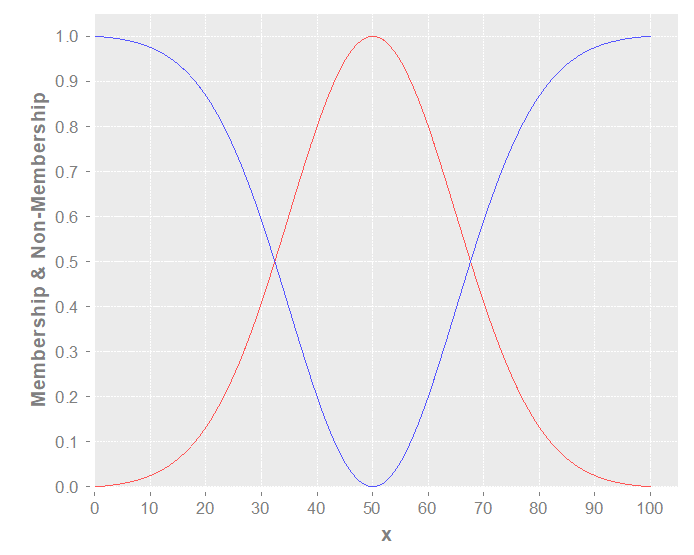
\includegraphics[width=0.7\textwidth]{img/traditional-set-as-ifs.png}
\label{figure:traditional-set-as-ifs}
\end{figure}

Figure \ref{figure:example-of-ifs} is the first case of an IFS that cannot be
considered a tradi-tional fuzzy set. The red line represents the membership
function, while the blue line represents the non-membership function. As can be
seen, the Gaussian membership function does not have a kernel, meaning that its
highest valued member does not equal to 1. In this case, its highest valued
member equals to 0.7, and for the non-membership function, its highest valued
member equals to 0.3. The Gaussian membership function is constructed with a
mean of 50 and a standard deviation of 15. For the non-membership function, it
is con-structed with a mean of 30 and standard deviation of 30.

\begin{figure}
\caption{Representation of an intuitionistic fuzzy set} \centering
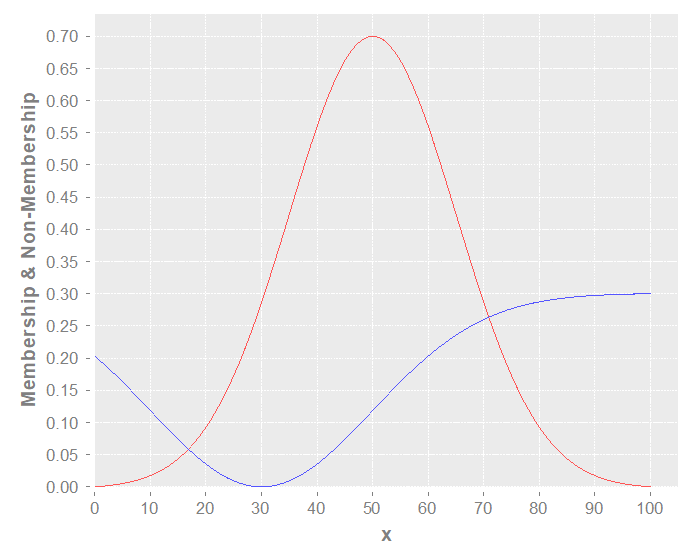
\includegraphics[width=0.7\textwidth]{img/example-of-ifs.png}
\label{figure:example-of-ifs}
\end{figure}
